\chapter{Experimental task 1 - IntelligentOffice - \tdd group}
\label{appendix:A_IntelligengOffice}
\section{Constraints}
Your project must be free of syntactic errors. Please make sure that your code actually runs in PyCharm.

\section{Task goal}
The goal of this task is to develop an intelligent office system, which allows the user to manage the light, blinds, and air quality level inside the office.
The office is square in shape and it is divided into four quadrants of equal dimension; on the ceiling of each quadrant lies an infrared (IR) distance sensor used to detect the presence of a worker inside that quadrant. 
The office has a wide window on one side of the upper left quadrant, equipped with a servo motor to open/close the blinds. 
Based on a Real Time Clock (RTC), the intelligent office system opens/closes the blinds each working day. 
A photoresistor, used to measure the light level inside the office, is placed on the ceiling. Based on the measured light level, the intelligent office system turns on/off a (ceiling-mounted) smart light bulb. 
Finally, the system also monitors the air quality in the office through a carbon dioxide (CO2) sensor and then regulates the air quality by controlling the switch of an exhaust fan.
To recap, the following sensors and actuators are present:

\begin{itemize}
    \item Four infrared distance sensors, one in each quadrant of the office.
    \item RTC to handle time operations.
    \item Servo motor to open/close the blinds of the office window.
    \item Photoresistor to measure the light level inside the office.
    \item Smart light bulb.
    \item Carbon dioxide sensor, used to measure the CO2 levels inside the office.
    \item Switch to control an exhaust fan mounted on the ceiling.
\end{itemize}

The communication between the main board and the other components happens with GPIO pins; GPIO communication is configured in BOARD mode. For further details on how to use the GPIO library refer to the \texttt{mock.GPIO} file in the source code.
Handle any error situation that you may encounter by throwing the \texttt{IntelligentOfficeError} exception.
Figure \ref{office_layout} recaps the layout of the sensors and actuators in the office.

\begin{figure}[H]
    \centering
    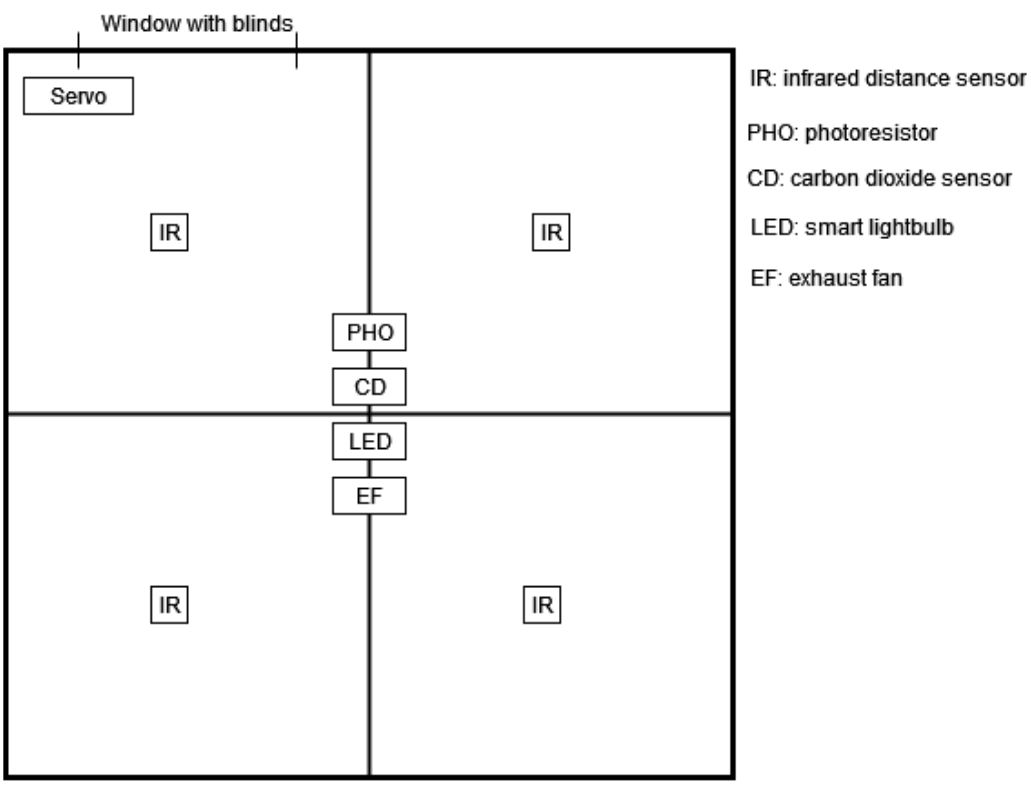
\includegraphics[width=\linewidth]{figures/appendix/intelligent_office.png}
    \caption{Office layout.}
    \label{office_layout.}
\end{figure}

For now, you don't need to know more; further details will be provided in the user stories below.

\section{Instructions}
Depending on your preference, either clone the repository at \url{https://github.com/Espher5/intelligent_office} or download the source files as a zip archive; afterwards, import the project into PyCharm. 
Take a look at the provided project, which contains the following classes: 
\begin{itemize}
    \item \textbf{\texttt{IntelligengOffice}}: you will implement your methods here.
    \item \textbf{\texttt{IntelligengOfficeError}}: exception that you will raise to handle errors.
    \item \textbf{\texttt{IntelligengOfficeTest}}: you will write your tests here.
    \item \textbf{\texttt{mock.GPIO}}: contains the mocked methods for GPIO functionalities.
    \item \textbf{\texttt{mock.RTC}}: contains the mocked methods for RTC functionalities.
\end{itemize}

Remember, you are not allowed to modify the provided API in any way (\ie class names, method names, parameter types, return types). You can however add fields, methods, or even classes (including other test classes), as long as you comply with the provided API. Use \tdd to implement this software system.
The requirements of the software system to be implemented are divided into a set of user stories, which serve as a to-do list; you should be able to incrementally develop the software system, without an upfront comprehension of all the requirements. Do not read ahead and handle the requirements (\ie specified in the user stories) one at a time in the order provided.
When a story is implemented, move on to the next one; a story is implemented when you are confident that your software system correctly implements all the functionality stipulated by the story's requirement. This implies that all your tests for that story and all the tests for the previous stories pass. You may need to review your software system as you progress towards more advanced requirements.
At the end of the task, fill out the post-questionnaire where, among other things, you will be asked to share your project (either as a link to a GitHub repository or as a public link to a zip file). The post-questionnaire is available at: \url{https://forms.gle/H4eNDDR6CjLjUofY6}.


\section{User Stories}
\subsection{Office worker detection}
Four infrared distance sensors, one in each office quadrant, are used to determine whether someone is currently in that quadrant.
Each sensor has a data pin connected to the board, used by the system in order to receive the measurements; more specifically, the four sensors are connected to pin 11, 12, 13, and 15, respectively (BOARD mode).
The communication with the sensors happens via the GPIO \texttt{input} function. The pins have already been set up in the constructor of the \texttt{IntelligentOffice} class. 
The output of the infrared sensor is an analog signal which changes intensity according to the distance between the sensor and the object (\ie 2.5V when an object is 50 cm away and ~0V when the object is out of the max range of the sensor). For this exercise, let's assume the input can be classified into just these two categories:
\begin{itemize}
    \item \textbf{Non-zero value}: it indicates that an object is present in front of the sensor (\ie a worker).
    \item \textbf{Zero value}: nothing is detected in front of the sensor.
\end{itemize}

\ \\ \
\noindent\textbf{Requirement}:
\begin{itemize}
    \item Implement \texttt{IntelligentOffice.check\_quadrant\_occupancy(pin: int) $\,\to\,$ bool} to verify whether a specific quadrant has someone inside it.
\end{itemize}


\subsection{Open/close blinds based on time}
Regardless of the presence of workers in the office, the intelligent office system fully opens the blinds at $8:00$ and fully closes them at $20:00$ each day except for Saturday and Sunday.
The system gets the current time and day from the RTC module connected on pin 16 (BOARD mode) which has already been set up in the constructor of  the \texttt{IntelligentOffice} class. Use the instance variable \texttt{self.rtc} and the methods of \texttt{mock.RTC} to retrieve these values.

To open/close the blinds, the system commands a servo motor, which is a type of DC (Direct Current) motor that, upon receiving a signal, can rotate itself to any angle from 0$^{\circ}$ to 180$^{\circ}$. We can control it by sending a Pulse-Width Modulation (PWM) signal to its signal pin; this means sending a HIGH signal for a certain period of time (called duty cycle), followed by a LOW signal period. The duty cycle determines the angle the servo motor will rotate to.

The servo is connected on pin 18 (BOARD mode), and operates at 50hz frequency. Furthermore, let's assume the blinds can be in the following states:
\begin{itemize}
    \item \textbf{Fully closed}, corresponding to a 0$^{\circ}$ rotation of the servo motor.
    \item \textbf{Fully open}, corresponding to a 180$^{\circ}$ rotation of the servo motor.
\end{itemize}

In order to calculate the duty cycle corresponding to a certain angle, refer to the following formula:
\[
    duty\_cycle = (angle / 18) + 2
\]
The servo motor has already been configured and can be controlled by passing the duty cycle (see the formula above) corresponding to the desired angle to the \texttt{change\_servo\_angle(duty\_cycle: float) $\,\to\,$ None }method in the \texttt{IntelligentOffice} class.
Finally, since at this stage of development there is no way to determine the state of the physical servo motor, use the \texttt{self.blinds\_open} instance variable to keep track of its state.

\ \\ \
\noindent\textbf{Requirement}:
\begin{itemize}
    \item Implement \texttt{IntelligentOffice.manage\_blinds\_based\_on\_time() $\,\to\,$ None} to control the behavior of the blinds.
\end{itemize}


\subsection{Light level management}
The intelligent office system allows setting a minimum and a maximum target light level in the office. The former is set to 500 lux, the latter to 550 lux. 
To meet the above-mentioned target light levels, the system turns on/off a smart light bulb. In particular, if the actual light level is lower than 500 lux, the system turns on the smart light bulb. On the other hand, if the actual light level is greater than 550 lux, the system turns off the smart light bulb. 

The actual light level is measured by the (ceiling-mounted) photoresistor connected on pin 22 (BOARD mode). The communication with the sensor happens via the GPIO \texttt{input} function. For this sensor, the value returned by the GPIO \texttt{input} function is assumed to be in lux. The pin has already been set up in the constructor of the \texttt{IntelligentOffice} class. 
The smart light bulb is represented by a LED, connected to the main board via pin 29 (BOARD mode). Communication with the LED happens via the GPIO \texttt{output} function. The pin has already been set up in the constructor of  the \texttt{IntelligentOffice} class.
Finally, since at this stage of development there is no way to determine the state of the physical light bulb, use the boolean instance variable \texttt{self.light\_on}, defined in the constructor of the \texttt{IntelligentOffice} class, to keep track of the state of the light bulb.

\ \\ \
\noindent\textbf{Requirement}:
\begin{itemize}
    \item Implement \texttt{IntelligentOffice.manage\_light\_level() $\,\to\,$ None} to control the behavior of the smart light bulb.
\end{itemize}


\subsection{Manage smart light bulb based on occupancy}
When the last worker leaves the office (\ie, the office is now vacant), the intelligent office system stops regulating the light level in the office and then turns off the smart light bulb. 
On the other hand, the intelligent office system resumes regulating the light level when the first worker goes back into the office. 

\ \\ \
\noindent\textbf{Requirement}:
\begin{itemize}
    \item Update the implementation of \texttt{IntelligentOffice.manage\_light\_level() $\,\to\,$ None} to control the behavior of the smart light bulb.
\end{itemize}


\subsection{Monitor air quality level}
A carbon dioxide sensor is used to monitor the CO2 levels inside the office. If the amount of detected CO2 is greater than or equal to 800 PPM, the system turns on the switch of the exhaust fan until the amount of CO2 is lower than 500 PPM.
The carbon dioxide sensor is connected on pin 31 (BOARD mode). The communication with the sensor happens via the GPIO \texttt{input} function. For this sensor, the value returned by the GPIO \texttt{input} function is assumed to be in PPM. 
The switch to the exhaust fan is connected on pin 32 (BOARD mode). The communication with the sensor happens via the GPIO \texttt{output} function.
Both the pin for the CO2 sensor and the one for the exhaust fan have already been set up in the constructor of the \texttt{IntelligentOffice} class. 
Finally, since at this stage of development there is no way to determine the state of the physical exhaust fan switch, use the boolean instance variable \texttt{self.fan\_switch\_on}, defined in the constructor of the \texttt{IntelligentOffice} class, to keep track of the state of the fan switch.

\ \\ \
\noindent\textbf{Requirement}:
\begin{itemize}
    \item Implement \texttt{IntelligentOffice.monitor\_air\_quality() $\,\to\,$ None} to control the behavior of CO2 sensor and the exhaust fan switch.
\end{itemize}
